\documentclass{article}
\usepackage[utf8]{inputenc}
\usepackage[a4paper, total={6in, 8in}]{geometry}
\usepackage{graphicx}
\usepackage{amsmath}
\usepackage{enumitem}
\usepackage{pgfplots}
\pgfplotsset{compat=1.18}
\title{ECON 20000 Problem Set 1}
\author{Ellis Garver}
\date{10/6/25}
\begin{document}
\maketitle
\item[] 
\textbf{Instructions:}
\begin{enumerate}
\item You need to submit your solutions to the problem set through gradescope. 
\item You need to submit your solutions individually. You are allowed to work in groups (at most 3), but you should each submit your own version of the solutions and write down the name(s) of group members on the top of your page.
\item Submissions are due Mondays at 6pm, late submissions are not accepted.
\item You can have handwritten or typed solutions. 
\end{enumerate}
 \textbf{Questions:}
\begin{enumerate}
\item For each function f(x) given below, compute the derivative df (x)/dx. Then find the critical point(s) of these functions, and use the sign of the second derivative to determine whether critical point(s) is a maximum or minimum.
\begin{enumerate}[label=(\alph*)]
\item $f(x) = -x^2 + 4x + 5$
\item[] $df(x)/dx=-2x+4,\;d^2f(x)/dx^2=-2$
\item[] $df(x)/dx=-2x+4=0 \Rightarrow\ 2x=4 \Rightarrow\ x=2$
\item[] $f(2)=-(2)^2+4(2)+5=9$
\item[] Critical point: (2,9) maximum
\item $f(x) = -x^4 + x^2 + 7$
\item[] $df(x)/dx=-4x^3+2x\;,\;d^2f(x)/dx^2=-12x^2+2$
\item[] $df(x)/dx=-4x^3+2x=0 \Rightarrow\ -2x(2x^2-1)=0 \Rightarrow\ x=0,\frac{1}{\sqrt{2}},\frac{-1}{\sqrt{2}}$
\item[] $f(0)=-(0)^4+(0)^2+7=7$ 
\item[] $f(\pm\frac{1}{\sqrt{2}})=-(\pm\frac{1}{\sqrt{2}})^4+(\pm\frac{1}{\sqrt{2}})^2+7=7.25$
\item[] $d^2f(0)/dx^2=2,\;d^2f(\pm\frac{1}{\sqrt{2}})/dx^2=-12(\pm\frac{1}{\sqrt{2}})^2+2=-12(\frac{1}{2})+2=-4$
\item[] Critical points: (0,7) minimum, ($\pm\frac{1}{\sqrt{2}},7.25$) maximum
\end{enumerate}
\item For the functions below, compute the partial derivatives both with respect to x and y. a and b are unknown, real-valued constants.
\begin{enumerate}[label=(\alph*)]
\item $f(x, y) = x^2 + axy -by^2$
\item[] $\partial f/\partial x=2x+ay$
\item[] $\partial f/\partial y=-2by+ax$
\item $f(x, y) = x^ay^b$
\item[] $\partial f/\partial x=y^bax^{a-1}$
\item[] $\partial f/\partial y=x^aby^{b-1}$
\item $f(x, y) =x^5+4\sqrt x+ln(x)+7y$
\item[] $\partial f/\partial x=5x^4 + \frac{2}{\sqrt{x}}+\frac{1}{x}$
\item[] $\partial f/\partial y=7$
\item $f(x, y) =\frac{3y}{2x^2}$
\item[] $\partial f/\partial x=-\frac{3y}{x^3}$
\item[] $\partial f/\partial y=\frac{3}{2x^2}$
\end{enumerate}
\item Calculate $\frac{dy}{dx}$ for the following functions using the implicit function theorem.
\begin{enumerate}[label=(\alph*)]
\item $ x^2y + 5y^3 = 8$
\item[] $f(x,y)=x^2y+5y^3-8=0$
\item[] $\partial f/\partial x=2xy$
\item[] $\partial f/\partial y=x^2+15y^2$
\item[] $dy/dx=-\frac{\partial f/\partial x}{\partial f/\partial y}=-\frac{2xy}{x^2+15y^2}$
\item $xy^2 + 2y = 0$
\item[] $f(x,y)=xy^2+2y=0$
\item[] $\partial f/\partial x=y^2$
\item[] $\partial f/\partial x=2xy+2$
\item[] $dy/dx=-\frac{\partial f/\partial x}{\partial f/\partial y}=-\frac{y^2}{2xy+2}$
\end{enumerate}
\item Question $3.1$ from Lima. You have \$60 to spend on food. You are interested in the nutritional content of the food, but you can't purchase carbs and proteins separately. You can buy steak and loaves of bread. You have the following price and nutrition information:
\begin{itemize}
    \item Steak costs \$6 a pound and one pound has 12 grams of protein and 6 grams of carbs.
    \item Loaves of bread cost \$5 a pound and one pound has 5 grams of protein and 15 grams of carbs.
\end{itemize}
\item[] Given this information, answer the following questions:
\begin{enumerate}
\item Derive the absolute price of a gram of protein.
\item[] The system can be described as
    \begin{cases}
        f(S): p_x12+p_y6=6 \\ f(B): p_x5+p_y15=5
    \end{cases}
\item[] where $p_x$ is the price of protein and $p_y$ is the price of carbs per gram. Solving for $p_x$:
\item[] $(-\frac{5}{2})f(S)+f(B)=-p_x30+p_x5-p_y15+p_y15=-15+5 \Rightarrow\ 10=p_x25\Rightarrow\ p_x=\$0.40$
\item Derive the absolute price of a gram of carbs.
\item[] If $p_x=\$0.40$, then using $f(B):0.40(5)+p_y15=5\Rightarrow\ p_y15=3\Rightarrow\ p_y=\$0.20$
\item At what rate can you exchange 1 gram of protein for 1 gram of carbs? Explain clearly how you obtain this number and explain what determines it.
\item[] Exchange rate: $\frac{\$0.40}{\$0.20}=2$. You can exchange 1 gram of protein for 2 grams of carbs. This is the real price and comes from the ratio of the absolute prices between protein/carbs.
\item If you spend all your money on loaves of bread, how many grams of carbs will you consume? How many grams of protein will you consume?
\item[] $\frac{\$60}{\$5}=12\text{ loaves of bread}$
\item[] $12\text{ loaves }*\;15\text{ grams of carbs per loaf}=180\text{ grams of carbs}$
\item[] $12\text{ loaves }*\;5\text{ grams of protein per loaf}=60\text{ grams of protein}$
\item If you spend all your money on steak, how many grams of carbs will you consume? How many grams of protein will you consume?
\item[] $\frac{\$60}{\$6}=10\text{ steaks}$
\item[] $10\text{ steaks }*\;6\text{ grams of carbs per steak}=60\text{ grams of carbs}$
\item[] $10\text{ steaks }*\;12\text{ grams of protein per steak}=120\text{ grams of protein}$
\item Derive the question of the individual's budget constraint.
\item[] True budget constraint (steak, bread): $p_bb+p_ss=m \Rightarrow\ 5b+6s= 60$, $s,b\geq0$
\item[] Budget constraint (nutrients): $p_xx+p_yy= m\Rightarrow\ 0.4x+0.2y= 60$, $x,y\geq0$
\item Draw the budget set. Make sure that you label all the relevant quantities.
\item[] 
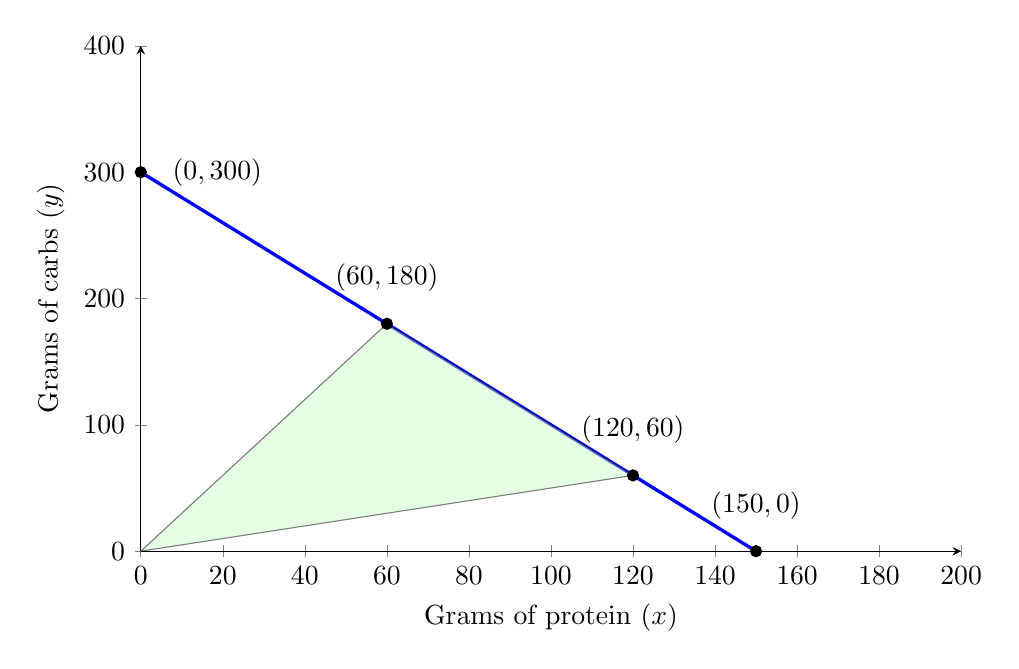
\begin{tikzpicture}
    \begin{axis} [
        axis lines = left,
        xlabel = {Grams of protein ($x$)},
        ylabel = {Grams of carbs ($y$)},
        xmin=0, xmax=200,
        ymin=0, ymax=400,
        width=12cm,
        height=8cm,
        grid=none,
        clip=false
    ]
        \addplot[very thick, blue] coordinates {(0,300)(150,0)};
        \addplot[fill=green!20, opacity=0.5] coordinates {(0,0)(120,60)(60,180)(0,0)};
        \addplot[mark=*, only marks] coordinates {(0,300)(150,0)};
        \addplot[mark=*, only marks] coordinates {(120,60)(60,180)};
        \node[above, yshift=8pt] at (axis cs:120,60) {$(120,60)$};
        \node[above, yshift=8pt] at (axis cs:60,180) {$(60,180)$};
        \node[right, xshift=8pt] at (axis cs:0,300) {$(0,300)$};
        \node[above, yshift=8pt] at (axis cs:150,0) {$(150,0)$};
    \end{axis}
\end{tikzpicture}
\end{enumerate}
\item(Quantity Discounts): Suppose Ricky buys only coffee and other goods. Harper Cafe decides to offer a discount to loyal patrons who buy more than 3 cups of coffee per day. The price of a cup of coffee is \$4 per cup for the first 3 cups, \$2 per cup for fourth and fifth cups and \$1 per cup for any cup after the fifth. Ricky limits himself to a budget of \$30 per day. The price of other goods is \$1 per unit.
\begin{enumerate}[label=(\alph*)]
\item Draw his budget constraint under this pricing scheme. Make sure you label the axes and the intercepts.
\item[] 
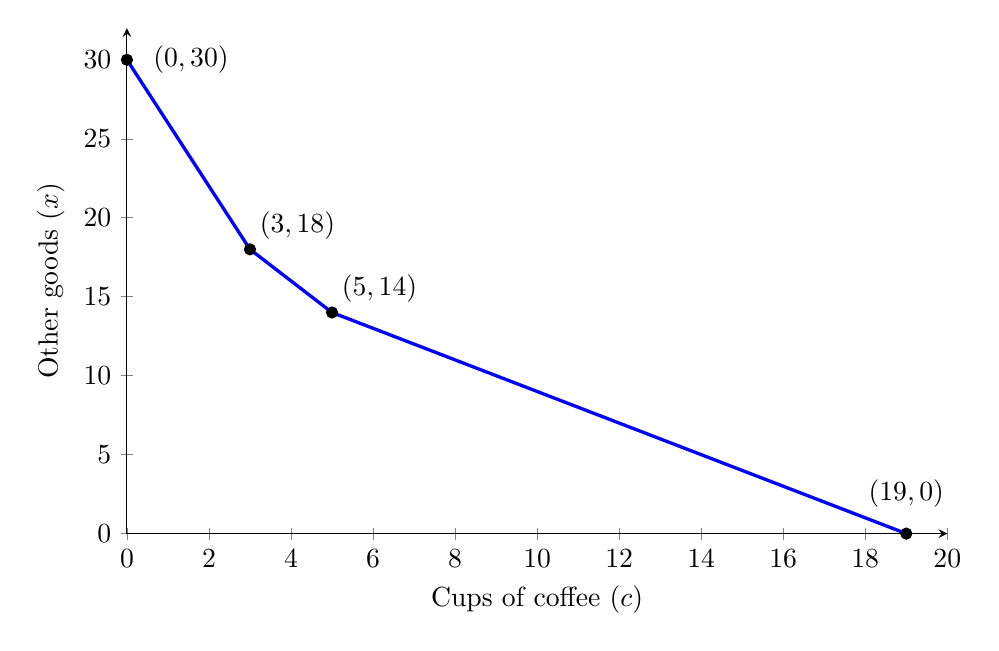
\begin{tikzpicture}
  \begin{axis}[
    axis lines = left,
    xlabel = {Cups of coffee ($c$)},
    ylabel = {Other goods ($x$)},
    xmin=0, xmax=20,
    ymin=0, ymax=32,
    width=12cm,
    height=8cm,
    grid=none,
    clip=false
  ]
    \addplot[very thick,blue] coordinates {(0,30)(3,18)(5,14)(19,0)};
    \addplot[mark=*, only marks] coordinates {(0,30) (3,18) (5,14) (19,0)};
    \node[right, xshift=6pt] at (axis cs:0,30) {$(0,30)$};
    \node[above right] at (axis cs:3,18) {$(3,18)$};
    \node[above right] at (axis cs:5,14) {$(5,14)$};
    \node[above, yshift=6pt] at (axis cs:19,0) {$(19,0)$};
  \end{axis}
\end{tikzpicture}
\item How many cups of coffee can Rick afford if he spends all his budget on coffee?
\item[] $\$30-\$4*3\;\text{cups}=\$18 \Rightarrow\ \$18-\$2*2\;\text{cups}=\$14 \Rightarrow\ \$14-\$1*14\;\text{cups}=0 \Rightarrow\ 19\; \text{cups}$
\item At what rate, can Ricky replace 1 cup of coffee with other goods (i.e. what is the opportunity cost of 1 cup of coffee in terms of other goods) if he consumes 2 cups of coffee per day?
\item[] 4 other goods per 1 cup of coffee
\item At what rate, can Ricky replace 1 cup of coffee with other goods (i.e. what is the opportunity cost of 1 cup of coffee in terms of other goods)  if he consumes 4 cups of coffee per day?
\item[] 2 other goods per 1 cup of coffee
\item At what rate, can Ricky replace 1 cup of coffee with other goods (i.e. what is the opportunity cost of 1 cup of coffee in terms of other goods)  if he consumes 6 cups of coffee per day?
\item[] 1 other good per 1 cup of coffee
\end{enumerate}
\end{enumerate}
\end{document}